% Graphic for TeX using PGF
% Title: C:\Users\CAMUGLIAL_INFO\Desktop\Diplome\Diplome\_Documentation\Diagrammes\Inscription.dia
% Creator: Dia v0.97.2
% CreationDate: Mon Jun 12 07:57:50 2017
% For: CAMUGLIAL_INFO
% \usepackage{tikz}
% The following commands are not supported in PSTricks at present
% We define them conditionally, so when they are implemented,
% this pgf file will use them.
\ifx\du\undefined
  \newlength{\du}
\fi
\setlength{\du}{15\unitlength}
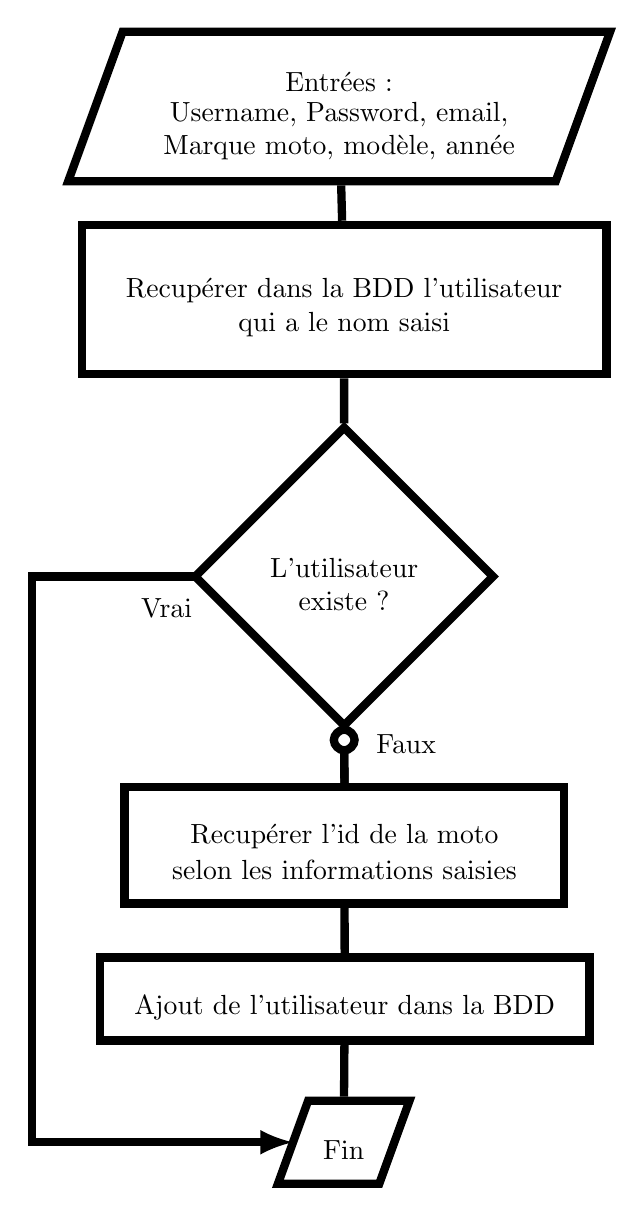
\begin{tikzpicture}
\pgftransformxscale{1.000000}
\pgftransformyscale{-1.000000}
\definecolor{dialinecolor}{rgb}{0.000000, 0.000000, 0.000000}
\pgfsetstrokecolor{dialinecolor}
\definecolor{dialinecolor}{rgb}{1.000000, 1.000000, 1.000000}
\pgfsetfillcolor{dialinecolor}
\definecolor{dialinecolor}{rgb}{1.000000, 1.000000, 1.000000}
\pgfsetfillcolor{dialinecolor}
\fill (22.186393\du,3.050000\du)--(33.929921\du,3.050000\du)--(32.619629\du,6.650000\du)--(20.876100\du,6.650000\du)--cycle;
\pgfsetlinewidth{0.200000\du}
\pgfsetdash{}{0pt}
\pgfsetdash{}{0pt}
\pgfsetmiterjoin
\definecolor{dialinecolor}{rgb}{0.000000, 0.000000, 0.000000}
\pgfsetstrokecolor{dialinecolor}
\draw (22.186393\du,3.050000\du)--(33.929921\du,3.050000\du)--(32.619629\du,6.650000\du)--(20.876100\du,6.650000\du)--cycle;
% setfont left to latex
\definecolor{dialinecolor}{rgb}{0.000000, 0.000000, 0.000000}
\pgfsetstrokecolor{dialinecolor}
\node at (27.403011\du,4.245000\du){Entrées :};
% setfont left to latex
\definecolor{dialinecolor}{rgb}{0.000000, 0.000000, 0.000000}
\pgfsetstrokecolor{dialinecolor}
\node at (27.403011\du,5.045000\du){Username, Password, email,};
% setfont left to latex
\definecolor{dialinecolor}{rgb}{0.000000, 0.000000, 0.000000}
\pgfsetstrokecolor{dialinecolor}
\node at (27.403011\du,5.845000\du){Marque moto, modèle, année };
\definecolor{dialinecolor}{rgb}{1.000000, 1.000000, 1.000000}
\pgfsetfillcolor{dialinecolor}
\fill (21.202200\du,7.700000\du)--(21.202200\du,11.300000\du)--(33.844700\du,11.300000\du)--(33.844700\du,7.700000\du)--cycle;
\pgfsetlinewidth{0.200000\du}
\pgfsetdash{}{0pt}
\pgfsetdash{}{0pt}
\pgfsetmiterjoin
\definecolor{dialinecolor}{rgb}{0.000000, 0.000000, 0.000000}
\pgfsetstrokecolor{dialinecolor}
\draw (21.202200\du,7.700000\du)--(21.202200\du,11.300000\du)--(33.844700\du,11.300000\du)--(33.844700\du,7.700000\du)--cycle;
% setfont left to latex
\definecolor{dialinecolor}{rgb}{0.000000, 0.000000, 0.000000}
\pgfsetstrokecolor{dialinecolor}
\node at (27.523450\du,9.295000\du){Recupérer dans la BDD l'utilisateur };
% setfont left to latex
\definecolor{dialinecolor}{rgb}{0.000000, 0.000000, 0.000000}
\pgfsetstrokecolor{dialinecolor}
\node at (27.523450\du,10.095000\du){qui a le nom saisi};
\definecolor{dialinecolor}{rgb}{1.000000, 1.000000, 1.000000}
\pgfsetfillcolor{dialinecolor}
\fill (27.523295\du,12.584100\du)--(31.108090\du,16.171934\du)--(27.523295\du,19.759768\du)--(23.938500\du,16.171934\du)--cycle;
\pgfsetlinewidth{0.200000\du}
\pgfsetdash{}{0pt}
\pgfsetdash{}{0pt}
\pgfsetmiterjoin
\definecolor{dialinecolor}{rgb}{0.000000, 0.000000, 0.000000}
\pgfsetstrokecolor{dialinecolor}
\draw (27.523295\du,12.584100\du)--(31.108090\du,16.171934\du)--(27.523295\du,19.759768\du)--(23.938500\du,16.171934\du)--cycle;
% setfont left to latex
\definecolor{dialinecolor}{rgb}{0.000000, 0.000000, 0.000000}
\pgfsetstrokecolor{dialinecolor}
\node at (27.523295\du,15.966934\du){L'utilisateur};
% setfont left to latex
\definecolor{dialinecolor}{rgb}{0.000000, 0.000000, 0.000000}
\pgfsetstrokecolor{dialinecolor}
\node at (27.523295\du,16.766934\du){ existe ?};
\definecolor{dialinecolor}{rgb}{1.000000, 1.000000, 1.000000}
\pgfsetfillcolor{dialinecolor}
\fill (22.235700\du,21.250000\du)--(22.235700\du,24.050000\du)--(32.825700\du,24.050000\du)--(32.825700\du,21.250000\du)--cycle;
\pgfsetlinewidth{0.200000\du}
\pgfsetdash{}{0pt}
\pgfsetdash{}{0pt}
\pgfsetmiterjoin
\definecolor{dialinecolor}{rgb}{0.000000, 0.000000, 0.000000}
\pgfsetstrokecolor{dialinecolor}
\draw (22.235700\du,21.250000\du)--(22.235700\du,24.050000\du)--(32.825700\du,24.050000\du)--(32.825700\du,21.250000\du)--cycle;
% setfont left to latex
\definecolor{dialinecolor}{rgb}{0.000000, 0.000000, 0.000000}
\pgfsetstrokecolor{dialinecolor}
\node at (27.530700\du,22.445000\du){Recupérer l'id de la moto};
% setfont left to latex
\definecolor{dialinecolor}{rgb}{0.000000, 0.000000, 0.000000}
\pgfsetstrokecolor{dialinecolor}
\node at (27.530700\du,23.245000\du){selon les informations saisies};
\definecolor{dialinecolor}{rgb}{1.000000, 1.000000, 1.000000}
\pgfsetfillcolor{dialinecolor}
\fill (21.644200\du,25.350000\du)--(21.644200\du,27.350000\du)--(33.431700\du,27.350000\du)--(33.431700\du,25.350000\du)--cycle;
\pgfsetlinewidth{0.200000\du}
\pgfsetdash{}{0pt}
\pgfsetdash{}{0pt}
\pgfsetmiterjoin
\definecolor{dialinecolor}{rgb}{0.000000, 0.000000, 0.000000}
\pgfsetstrokecolor{dialinecolor}
\draw (21.644200\du,25.350000\du)--(21.644200\du,27.350000\du)--(33.431700\du,27.350000\du)--(33.431700\du,25.350000\du)--cycle;
% setfont left to latex
\definecolor{dialinecolor}{rgb}{0.000000, 0.000000, 0.000000}
\pgfsetstrokecolor{dialinecolor}
\node at (27.537950\du,26.545000\du){Ajout de l'utilisateur dans la BDD};
\definecolor{dialinecolor}{rgb}{1.000000, 1.000000, 1.000000}
\pgfsetfillcolor{dialinecolor}
\fill (26.656040\du,28.800000\du)--(29.097217\du,28.800000\du)--(28.369276\du,30.800000\du)--(25.928100\du,30.800000\du)--cycle;
\pgfsetlinewidth{0.200000\du}
\pgfsetdash{}{0pt}
\pgfsetdash{}{0pt}
\pgfsetmiterjoin
\definecolor{dialinecolor}{rgb}{0.000000, 0.000000, 0.000000}
\pgfsetstrokecolor{dialinecolor}
\draw (26.656040\du,28.800000\du)--(29.097217\du,28.800000\du)--(28.369276\du,30.800000\du)--(25.928100\du,30.800000\du)--cycle;
% setfont left to latex
\definecolor{dialinecolor}{rgb}{0.000000, 0.000000, 0.000000}
\pgfsetstrokecolor{dialinecolor}
\node at (27.512658\du,29.995000\du){Fin};
\pgfsetlinewidth{0.200000\du}
\pgfsetdash{}{0pt}
\pgfsetdash{}{0pt}
\pgfsetmiterjoin
\pgfsetbuttcap
{
\definecolor{dialinecolor}{rgb}{0.000000, 0.000000, 0.000000}
\pgfsetfillcolor{dialinecolor}
% was here!!!
\pgfsetarrowsend{latex}
{\pgfsetcornersarced{\pgfpoint{0.000000\du}{0.000000\du}}\definecolor{dialinecolor}{rgb}{0.000000, 0.000000, 0.000000}
\pgfsetstrokecolor{dialinecolor}
\draw (23.938500\du,16.171900\du)--(20.000000\du,16.171900\du)--(20.000000\du,29.800000\du)--(26.292100\du,29.800000\du);
}}
\pgfsetlinewidth{0.200000\du}
\pgfsetdash{}{0pt}
\pgfsetdash{}{0pt}
\pgfsetbuttcap
{
\definecolor{dialinecolor}{rgb}{0.000000, 0.000000, 0.000000}
\pgfsetfillcolor{dialinecolor}
% was here!!!
\definecolor{dialinecolor}{rgb}{0.000000, 0.000000, 0.000000}
\pgfsetstrokecolor{dialinecolor}
\draw (27.452204\du,6.749280\du)--(27.474257\du,7.600720\du);
}
\pgfsetlinewidth{0.200000\du}
\pgfsetdash{}{0pt}
\pgfsetdash{}{0pt}
\pgfsetbuttcap
{
\definecolor{dialinecolor}{rgb}{0.000000, 0.000000, 0.000000}
\pgfsetfillcolor{dialinecolor}
% was here!!!
\definecolor{dialinecolor}{rgb}{0.000000, 0.000000, 0.000000}
\pgfsetstrokecolor{dialinecolor}
\draw (27.523450\du,9.500000\du)--(27.523450\du,9.500000\du);
}
\pgfsetlinewidth{0.200000\du}
\pgfsetdash{}{0pt}
\pgfsetdash{}{0pt}
\pgfsetbuttcap
{
\definecolor{dialinecolor}{rgb}{0.000000, 0.000000, 0.000000}
\pgfsetfillcolor{dialinecolor}
% was here!!!
\definecolor{dialinecolor}{rgb}{0.000000, 0.000000, 0.000000}
\pgfsetstrokecolor{dialinecolor}
\draw (27.523406\du,11.400100\du)--(27.523381\du,12.484101\du);
}
\pgfsetlinewidth{0.200000\du}
\pgfsetdash{}{0pt}
\pgfsetdash{}{0pt}
\pgfsetbuttcap
{
\definecolor{dialinecolor}{rgb}{0.000000, 0.000000, 0.000000}
\pgfsetfillcolor{dialinecolor}
% was here!!!
\definecolor{dialinecolor}{rgb}{0.000000, 0.000000, 0.000000}
\pgfsetstrokecolor{dialinecolor}
\draw (27.533639\du,24.149963\du)--(27.535796\du,25.250659\du);
}
\pgfsetlinewidth{0.200000\du}
\pgfsetdash{}{0pt}
\pgfsetdash{}{0pt}
\pgfsetbuttcap
{
\definecolor{dialinecolor}{rgb}{0.000000, 0.000000, 0.000000}
\pgfsetfillcolor{dialinecolor}
% was here!!!
\definecolor{dialinecolor}{rgb}{0.000000, 0.000000, 0.000000}
\pgfsetstrokecolor{dialinecolor}
\draw (27.529892\du,27.449182\du)--(27.520716\du,28.700818\du);
}
% setfont left to latex
\definecolor{dialinecolor}{rgb}{0.000000, 0.000000, 0.000000}
\pgfsetstrokecolor{dialinecolor}
\node[anchor=west] at (22.310700\du,16.942500\du){Vrai};
% setfont left to latex
\definecolor{dialinecolor}{rgb}{0.000000, 0.000000, 0.000000}
\pgfsetstrokecolor{dialinecolor}
\node[anchor=west] at (27.978400\du,20.200400\du){Faux};
\pgfsetlinewidth{0.200000\du}
\pgfsetdash{}{0pt}
\pgfsetdash{}{0pt}
\pgfsetbuttcap
{
\definecolor{dialinecolor}{rgb}{0.000000, 0.000000, 0.000000}
\pgfsetfillcolor{dialinecolor}
% was here!!!
\definecolor{dialinecolor}{rgb}{0.000000, 0.000000, 0.000000}
\pgfsetstrokecolor{dialinecolor}
\draw (27.523300\du,19.759800\du)--(27.530700\du,21.250000\du);
}
\definecolor{dialinecolor}{rgb}{0.000000, 0.000000, 0.000000}
\pgfsetstrokecolor{dialinecolor}
\draw (27.526279\du,20.359793\du)--(27.530700\du,21.250000\du);
\pgfsetlinewidth{0.200000\du}
\pgfsetdash{}{0pt}
\pgfsetmiterjoin
\pgfsetbuttcap
\definecolor{dialinecolor}{rgb}{1.000000, 1.000000, 1.000000}
\pgfsetfillcolor{dialinecolor}
\pgfpathmoveto{\pgfpoint{27.523797\du}{19.859799\du}}
\pgfpathcurveto{\pgfpoint{27.648795\du}{19.859178\du}}{\pgfpoint{27.774414\du}{19.983556\du}}{\pgfpoint{27.775035\du}{20.108554\du}}
\pgfpathcurveto{\pgfpoint{27.775656\du}{20.233553\du}}{\pgfpoint{27.651278\du}{20.359172\du}}{\pgfpoint{27.526279\du}{20.359793\du}}
\pgfpathcurveto{\pgfpoint{27.401281\du}{20.360413\du}}{\pgfpoint{27.275662\du}{20.236036\du}}{\pgfpoint{27.275041\du}{20.111037\du}}
\pgfpathcurveto{\pgfpoint{27.274420\du}{19.986039\du}}{\pgfpoint{27.398798\du}{19.860419\du}}{\pgfpoint{27.523797\du}{19.859799\du}}
\pgfusepath{fill}
\definecolor{dialinecolor}{rgb}{0.000000, 0.000000, 0.000000}
\pgfsetstrokecolor{dialinecolor}
\pgfpathmoveto{\pgfpoint{27.523797\du}{19.859799\du}}
\pgfpathcurveto{\pgfpoint{27.648795\du}{19.859178\du}}{\pgfpoint{27.774414\du}{19.983556\du}}{\pgfpoint{27.775035\du}{20.108554\du}}
\pgfpathcurveto{\pgfpoint{27.775656\du}{20.233553\du}}{\pgfpoint{27.651278\du}{20.359172\du}}{\pgfpoint{27.526279\du}{20.359793\du}}
\pgfpathcurveto{\pgfpoint{27.401281\du}{20.360413\du}}{\pgfpoint{27.275662\du}{20.236036\du}}{\pgfpoint{27.275041\du}{20.111037\du}}
\pgfpathcurveto{\pgfpoint{27.274420\du}{19.986039\du}}{\pgfpoint{27.398798\du}{19.860419\du}}{\pgfpoint{27.523797\du}{19.859799\du}}
\pgfusepath{stroke}
\end{tikzpicture}
